\chapter{Construcción aplicaciones}
\label{cap:Construccion}

Este capítulo detalla la fase de construcción de la aplicación, comenzando con la toma de requistos, la toma de desiciones de diseño y culmina con la implementación.

\section{Toma de requisitos}
\label{sec:Requisitos}

Se han construido dos aplicaciones; La primera es el visualizador, el que se encarga de aplicar los filtros y mostrar la información correspondiente a los puntos donde se han detectado necesidades y la segunda corresponde a aquella que realiza la recepción del flujo de datos desde \textit{Twitter} y su paso por el clasificador. Las razones por las que se consideraron dos aplicaciones separadas se especificarán en la sección \ref{sec:Diseno}. A continuación se presenta el proceso de diseño y construcción de cada una de ellas.

\subsection{Visualizador}
\label{subsec:ReqVisualizador}

En conversaciones con los profesores guía y co-guía del presente trabajo - Clientes - se señaló que se requería un visualizador en el que se mostraran las necesidades recogidas desde \textit{Twitter}. Para ello se sugirió utilizar un mapa en el cual se señalara mediante marcadores los puntos en cuestión, de modo que éste fue el punto inicial.\\

La Tabla ~\ref{tab:ReqVi}. lista las historias de usuario que representan los requisitos identificados en el presente. Estas hisotorias tienen un ID y una descripción, donde el ID se compone de "HU-vXX", haciendo referencia a que corresponde al visualizador, donde 'XX' corresponde al número del requisito.\\

\begin{table}[]
\centering
\caption{Tabla de historias de usuario.}
\label{tab:ReqVi}
\begin{tabular}{|c|l|}
\hline
ID & \multicolumn{1}{c|}{Descripción} \\ \hline
HU-v01 & \begin{tabular}[c]{@{}l@{}}Como usuario quiero visualizar las necesidades expresadas\\ como un punto en un mapa geográfico del país.\end{tabular} \\ \hline
HU-v02 & \begin{tabular}[c]{@{}l@{}}Como usuario quiero poder filtrar qué necesidades mostrar\\  en cada momento según su categoría.\end{tabular} \\ \hline
HU-v03 & \begin{tabular}[c]{@{}l@{}}Como usuario quiero que, según el nivel de acercamiento \\ del mapa, los puntos se agrupen.\end{tabular} \\ \hline
HU-v04 & \begin{tabular}[c]{@{}l@{}}Como usuario quiero que el agrupamiento pueda realizarse\\ según su categoría en lugar de su proximidad.\end{tabular} \\ \hline
HU-v05 & \begin{tabular}[c]{@{}l@{}}Como usuario quiero seleccionar un intervalo de tiempo y \\ que se muestren los puntos identificados dentro de ese \\ intervalo.\end{tabular} \\ \hline
HU-v06 & \begin{tabular}[c]{@{}l@{}}Como usuario quiero poder especificar términos para la\\ búsqueda de necesidades.\end{tabular} \\ \hline
HU-v07 & \begin{tabular}[c]{@{}l@{}}Como usuario quiero que los parámetros para el \\ funcionamiento del sistema sean modificables.\end{tabular} \\ \hline
HU-v08 & \begin{tabular}[c]{@{}l@{}}Como usuario quiero que se muestre la nomenclatura de\\ los íconos que son mostrados en el mapa.\end{tabular} \\ \hline
HU-v08 & \begin{tabular}[c]{@{}l@{}}Como usuario quiero que se visualicen estadísticas sobre\\ la cantidad de elementos procesados como por ejemplo: \\ cantidad de tweets, necesidades detectadas y cantidad de \\ usuarios diferentes.\end{tabular} \\ \hline
\end{tabular}
\end{table}

Estos requisitos no fueron producto de sólo una reunión con los clientes, sino que son producto de una serie de demostraciones de la aplicación, sugeridos como cambios deseables a la aplicación y fueron considerados de acuerdo a la metodología.\\

\subsection{Clasificador}
\label{subsec:ReqClasificador}

Como parte de la aplicación la función del clasificador se pensó desde el primer momento el ser soportado por Apache Storm, aquel fue el punto de inicio; La aplicación internamente tendría forma de grafo y cada nodo de aquel grafó — \textit{Bolt} — realizará una tarea específica.\\

Dentro de la metodología KDD, como se señaló en la sección ~\ref{subsec:kdd} un paso de preprocesamiento de los datos, por lo que se consideró que la información proveniente desde \textit{Twitter} debería sufrir el mismo preprocesamiento que señala \ref{tenicasKDD}. Según lo anteriormente descrito se originan los requisitos que dan como resultado las historias de usuario que se presentan en la Tabla ~\ref{tab:ReqClas}. Junto con la descripción la ID de la historía tendrá la siguiente forma: "HU-cXX", donde 'XX' corresponde al número del requisito.\\

\begin{table}[]
\centering
\caption{Requisitos del clasificador.}
\label{tab:ReqClas}
\begin{tabular}{|l|l|}
\hline
\multicolumn{1}{|c|}{ID} & \multicolumn{1}{c|}{Descripción}                                                                                                                               \\ \hline
HU-c01                   & \begin{tabular}[c]{@{}l@{}}Como cliente quiero que la aplicación esté soportada sobre\\ Apache Storm.\end{tabular}                                             \\ \hline
HU-c02                   & \begin{tabular}[c]{@{}l@{}}Como cliente quiero que la aplicación recoja el flujo de\\ datos de Twitter.\end{tabular}                                           \\ \hline
HU-c03                   & \begin{tabular}[c]{@{}l@{}}Como cliente quiero que se apliquen los filtros descritos en\\ la literatura.\end{tabular}                                          \\ \hline
HU-c04                   & \begin{tabular}[c]{@{}l@{}}Como cliente quiero que se consiga la ubicación desde \\ dónde se originó el Tweet o del lugar al que hace referencia.\end{tabular} \\ \hline
HU-c05                   & \begin{tabular}[c]{@{}l@{}}Como cliente quiero conocer la necesidad a la que el Tweet \\ hace referencia, si es que lo hace.\end{tabular}                      \\ \hline
\end{tabular}
\end{table}

\section{Desiciones de diseño}
\label{sec:Diseno}

Como se mencionó en la sección anterior, se haría uso de Apache Storm como \textit{framework} de computación distribuida para asegurar la escalabilidad del sistema. Dado el uso de Apache Storm (Con su versión 0.10 disponible al momento de la realización de este trabajo), la elaboración de una aplicación única que realizase ambas labores: procesar y visualizar, se dificultaba, dado que la aplicación que utilizase Storm como base requería ser ejecutada utilizando la aplicación distribuída por Apache además de Zookeeper, mientras que para implementar una aplicación web requeriría utilizar un servidor de aplicaciones. Es por ello que se decidió elaborar dos aplicaciones que, en conjunto, suplieran las necesidades del cliente.\\

Teniendo claro que consistiría de dos aplicaciones separadas surgía el problema de cómo realizar la comunicación entre ellas.\\

Por el lado del visualizador \textit{web} restaba saber qué \textit{framework} sería el más apropiado para su desarrollo. Dado que el equipo de desarrollo está limitado a una persona se pensó en un \textit{framework} que permitiera agilizar el proceso de desarrollo; por ello en lugar de otro se consideró el uso de \textit{Play Framework}, dado su enfoque en equipos de desarrollo ágil y su rapidez para visualizar los cambios del código \ref{playFramework}.\\

En un primer momento se pensó en realizar la comunicación REST dado que las aplicaciones desarrolladas mediante \textit{Play Framework} son, por defecto, RESTful, mas no se consideró implementar persistencia en los datos para que pudiesen ser considerados con posterioridad. Luego de discutir el diseño con los clientes se llego a la conclusión que la implementación de un sistema de base de datos permitiría elaborar la historia de usuario HU-v05.\\

Finalmente restaba seleccionar qué motor de base de datos. Se pensó en MySQL en primer lugar dado su familiaridad y simplicidad, pero se desechó al considerar que se trabajará con grandes cantidados de datos lo que involucrará muchas operaciones IO de escritura y lectura; dato el trabajo presentado en \ref{comparacionDBMS} además de la información de rendimiento presentada en \ref{mongoScale}, se seleccionó MongoDB como base de datos para el sistema.\\

Teniendo ya todos los elementos para construir la aplicación se presentó la arquitectura presente en la Figura ~\ref{fig:arquitecturaGeneral}. En ella se aprecia que através de la API de \textit{Twitter} la aplicación "Clasificador" (siendo ejecutara dobre Storm), recibe el \textit{stream} para posteriormente procesarlo y almacenarlo dentro de la base de datos. Por su parte el "Visualizador" recoge la información desde la base de datos y la muestra por pantalla. Además es posible pasarle términos de búsqueda al clasificador haciendo uso de la misma base de datos. \\

	\begin{figure}[H]
		\centering
		\captionsetup{justification=centering}
		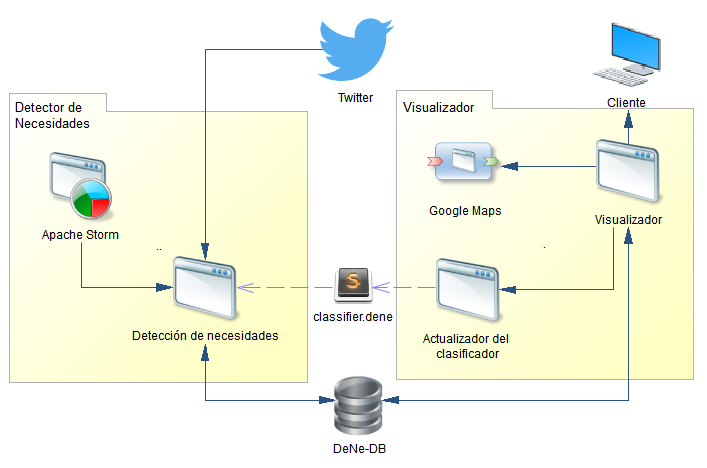
\includegraphics[scale=0.8]{images/arquitecturaGeneral.png}
		\caption[Arquitectura general del sistema.]{Arquitectura general del sistema.}
		\label{fig:arquitecturaGeneral}
	\end{figure}


Si bien no es necesario, se definieron dos esquemas para almacenar la información en la base de datos: El primero corresponde al esquema que tendrá la información guardada por el clasificador correspondiente a los marcadores y la segunda corresponde a las consultas realizadas desde el visualizador como términos para filtrar la búsqueda dentro del \textit{stream}. Dichos esquemas pueden ser apreciados en los ejemplos presentados en las Figuras ~\ref{fig:Marker} y ~\ref{fig:Query}, respectivamente.\\


\begin{figure}[H]
	\centering
	\captionsetup{justification=centering}
	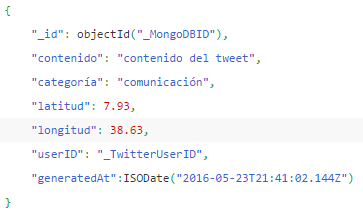
\includegraphics[scale=0.8]{images/marker.png}
	\caption[Ejemplo de documento en la colección Markers.]{Ejemplo de documento en la colección Markers.}
	\label{fig:Marker}
\end{figure}

Donde "id" corresponde a la ID generada por MongoDB al almacenar el documento, "contenido" corresponde al texto original del \textit{Tweet}, "categoría" corresponde, como su nombre lo señala, a la categoría a la que pertenece (agua, alimento, electricidad, comunicación, personas, seguridad o irrelevante), "latitud" y "longitud" corresponden a las coordenadas geográficas decimales donde se ubica el marcador, "userID" corresponde al ID del usuario que emitió ese \textit{Tweet} y, finalmente, "generatedAt" al \textit{timestamp} de cuándo fue generado ese marcador.\\

\begin{figure}[H]
	\centering
	\captionsetup{justification=centering}
	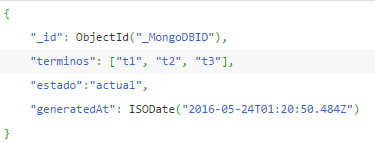
\includegraphics[scale=0.8]{images/query.png}
	\caption[Ejemplo de documento en la colección Markers.]{Ejemplo de documento en la colección Markers.}
	\label{fig:Query}
\end{figure}

De igual manera que en el documento de marcador, "id" corresponde a la ID generada por MongoDB al almacenar, "terminos" corresponde a un arreglo de \textit{string} que almacena los términos de búsqueda para filtrar el \textit{stream} de entrada, "estado" puede tomar dos valores: "actual" o "antigua" y sirve para señalar si se debe o no filtrar por los términos del documento. Finalmente "generatedAt" corresponde al \textit{timestamp} de cuándo fué originada esa consulta.\\







